% begin module implicit-tangent-line
%\abovedisplayskip=0pt
%\belowdisplayskip=0pt
%\abovedisplayshortskip=0pt
%\belowdisplayshortskip=0pt
\begin{frame}
\begin{example}
Find an equation of the tangent line to $(x-1)^2 + (y+2)^2 = 25$ at $(-2,2)$.
\begin{columns}
\column{0.35\textwidth}
\psset{xunit=0.25cm, yunit=0.25cm}
\begin{pspicture}(-6, -7.5)(6.9,4)
\tiny
\fcBoundingBox{-5}{-7.5}{6.5}{4}
\fcAxesStandard{-4.7}{-7.5}{6.5}{3.8}
\fcLabels{6.5}{3.8}
%\fcXTickWithLabel{-2.5}{$-2.5$}
\fcXTickWithLabel{5}{$5$}
\fcYTickWithLabel{-5}{$-5$}
%Function formula: -2- (\sqrt{25- ((-1+x)^{2})})
\psplot[linecolor=\fcColorGraph, plotpoints=1000]{-4}{6}{x -1 add 2 exp -1 mul 25 add sqrt -1 mul -2 add }
%Function formula: -2+\sqrt{25- ((-1+x)^{2})}
\psplot[linecolor=\fcColorGraph, plotpoints=1000]{-4}{6}{x -1 add 2 exp -1 mul 25 add sqrt -2 add }
\fcFullDot{-2}{2}
\rput[br](-1.9, 2.3){$(-2, 2)$}
\uncover<19->{
\psline[linecolor=\fcColorTangent](-4.666666667,0)(0.2,3.65)
}
\end{pspicture} %\only<handout:0|-15>{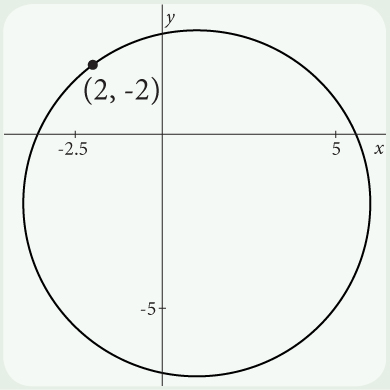
\includegraphics[height=3cm]{implicit-differentiation/pictures/implicit-tangent-linea.jpg}}
%\only<16->{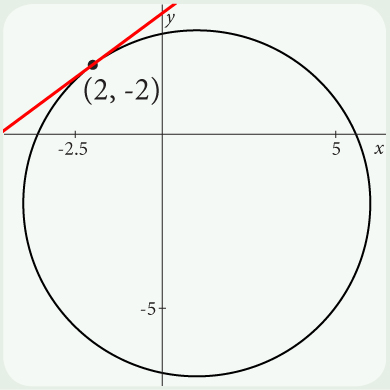
\includegraphics[height=3cm]{implicit-differentiation/pictures/implicit-tangent-lineb.jpg}}
\begin{align*}
\uncover<16->{&\text{Plug in } (\alertNoH{16,20}{-2},\alertNoH{17,19}{2}):}\\
\uncover<16->{&\frac{\diff y}{\diff x}  = \frac{1- (\alertNoH{16}{-2})}{\alertNoH{17}{2}+2}\uncover<18->{ = \alertNoH{21}{\frac{3}{4}}}}\\
\uncover<19->{&\text{Point-slope form:}\\
&y-\alertNoH{19}{2} = \alertNoH{21}{\frac{3}{4}} (x+\alertNoH{20}{2})}
\end{align*}
\column{0.65\textwidth}
\!\!\!\!\!\!\!\!\!\!\!\!\!\!\!$
\renewcommand{\arraystretch}{1.8}
\begin{array}{@{}r@{~}c@{~}l}
\displaystyle \uncover<2->{\text{Find} \ \frac{\diff y}{\diff x}, \ \text{given} \ (x-1)^2 \ + (y+2)^2 & =& 25:} \\
\uncover<3->{\displaystyle  \alertNoH{3-4}{\frac{\diff}{\diff x}\left((x-1)^2\right)} + \alertNoH{5-6}{\frac{\diff}{\diff x}\left((y+2)^2\right)}   &=&\displaystyle \alertNoH{7-8}{ \frac{\diff}{\diff x}(25)}}\\
\uncover<3->{\displaystyle  \fcAnswerUncover{3}{4}{2(x-1)\alertNoH{9}{\frac{\diff}{\diff x}(x-1)}} +\fcAnswerUncover{3}{6}{ 2(y+2)\alertNoH{11-12}{ \frac{\diff}{\diff x}(y+2) }}  &=& \fcAnswerUncover{3}{8}{0}}\\
\uncover<9->{\displaystyle  \alertNoH{13}{ 2(\alertNoH{14}{x-1}) \alertNoH{9-10} {(\fcAnswerUncover{9}{10}{1})}} + 2(y+2)\alertNoH{11-12}{\left( \fcAnswerUncover{9}{12}{\frac{\diff y}{\diff x}} \right)}  & =& 0}\\
\uncover<13->{\displaystyle   2\alertNoH{15}{(y+2)}\left( \frac{\diff y}{\diff x} \right) & = &\displaystyle \alertNoH{13}{2(\alertNoH{14}{1-x} )}}\\
\uncover<15->{\displaystyle  \frac{\diff y}{\diff x} &= &\displaystyle \frac{1-\alertNoH{16}{x}}{\alertNoH{15}{ \alertNoH{17}{y}+2}}}
\end{array}
$
\end{columns}
\end{example}
\end{frame}
% end module implicit-tangent-line
